\documentclass{amsart}

\usepackage{graphicx}

\newtheorem{theorem}{Theorem}[section]
\newtheorem{lemma}[theorem]{Lemma}

\theoremstyle{definition}
\newtheorem{definition}[theorem]{Definition}
\newtheorem{example}[theorem]{Example}
\newtheorem{xca}[theorem]{Exercise}

\theoremstyle{remark}
\newtheorem{remark}[theorem]{Remark}

\numberwithin{equation}{section}

%    Absolute value notation
\newcommand{\abs}[1]{\lvert#1\rvert}

%    Blank box placeholder for figures (to avoid requiring any
%    particular graphics capabilities for printing this document).
\newcommand{\blankbox}[2]{%
  \parbox{\columnwidth}{\centering
%    Set fboxsep to 0 so that the actual size of the box will match the
%    given measurements more closely.
    \setlength{\fboxsep}{0pt}%
    \fbox{\raisebox{0pt}[#2]{\hspace{#1}}}%
  }%
}

\begin{document}

\title{A Proposed Neural Network Activation Function}

\author{Matthew Schroeder}

\date{March 11, 2019}

\begin{abstract}
In this paper a new activation function for deep neural networks is presented.  Their are two variants of the activation function. The first is a smooth, oscillatory version of ReLU. The second is a smooth, oscillatory version of ReLU with exponential decay of the oscillations.
\end{abstract}

\maketitle

\section{INTRODUCTION}
The primary reason neural networks are so successful at solving problems in machine learning is their ability to create highly non-linear functions.   The feature of a neural network which makes this possible is the activation function.  The activation function takes what is otherwise a linear and makes it into a non-linear object.  It is no surprise then, that discovering new activation functions to use in neural networks is an ongoing area of research.   

The most popular activation function used today is the rectified linear unit (ReLU).  The most attractive property of ReLU seems to be its simplicity; the computation of this function is very fact, which simplifies and accelerates the training of neural networks. ReLU, however, is not differentiable at the origin, which has lead to the search for other activation function which are and have similar properties to ReLU.  The purpose of this paper is to present two more.    

While writing software to control servo hydraulic actuators, I was looking for a way to ramp the position of the actuator between two points.  The obvious choice is a line: $$f(x) = ax+b$$ Unfortunately, this is not differentiable, and so there are sudden changes in velocity which may damage the specimen attached to the actuator.  The standard way in the industry is to use a haversine, whose formula is given by $$f(x) = \frac{1-cos(x)}{2}$$  This function, however, is only $\mathscr{C}^1$, and sudden changes in acceleration can also be detrimental.  This lead me to consider the function $$f(x) = x - sin(x)$$  Here we have 'ramp' which is $\mathscr{C}^2$.   The third derivative is the jerk, and specimens seem to be able to tolerate discontinuities in the jerk.   See Fig. 1 for the graph of these three functions.

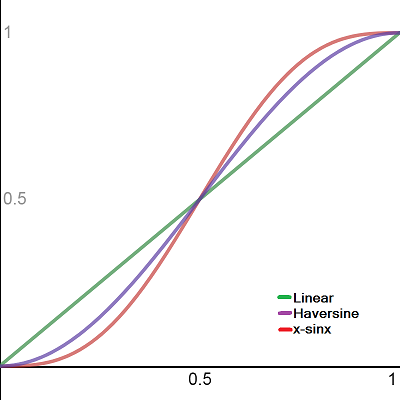
\includegraphics[1]{All_three.png}
\caption{Fig. 1: Three ramp functions.}



whose formula is given by $$f(x) = max(0,x)$$

\begin{lemma}
Let $f, g\in  A(X)$ and let $E$, $F$ be cozero
sets in $X$.
\begin{enumerate}
\item If $f$ is $E$-regular and $F\subseteq E$, then $f$ is $F$-regular.

\item If $f$ is $E$-regular and $F$-regular, then $f$ is $E\cup
F$-regular.

\item If $f(x)\ge c>0$ for all $x\in E$, then $f$ is $E$-regular.

\end{enumerate}
\end{lemma}

The following is an example of a proof.

\begin{proof} Set $j(\nu)=\max(I\backslash a(\nu))-1$. Then we have
\[
\sum_{i\notin a(\nu)}t_i\sim t_{j(\nu)+1}
  =\prod^{j(\nu)}_{j=0}(t_{j+1}/t_j).
\]
Hence we have
\begin{equation}
\begin{split}
\prod_\nu\biggl(\sum_{i\notin
  a(\nu)}t_i\biggr)^{\abs{a(\nu-1)}-\abs{a(\nu)}}
&\sim\prod_\nu\prod^{j(\nu)}_{j=0}
  (t_{j+1}/t_j)^{\abs{a(\nu-1)}-\abs{a(\nu)}}\\
&=\prod_{j\ge 0}(t_{j+1}/t_j)^{
  \sum_{j(\nu)\ge j}(\abs{a(\nu-1)}-\abs{a(\nu)})}.
\end{split}
\end{equation}
By definition, we have $a(\nu(j))\supset c(j)$. Hence, $\abs{c(j)}=n-j$
implies (5.4). If $c(j)\notin a$, $a(\nu(j))c(j)$ and hence
we have (5.5).
\end{proof}

\begin{quotation}
This is an example of an `extract'. The magnetization $M_0$ of the Ising
model is related to the local state probability $P(a):M_0=P(1)-P(-1)$.
The equivalences are shown in Table~\ref{eqtable}.
\end{quotation}

\begin{table}[ht]
\caption{}\label{eqtable}
\renewcommand\arraystretch{1.5}
\noindent\[
\begin{array}{|c|c|c|}
\hline
&{-\infty}&{+\infty}\\
\hline
{f_+(x,k)}&e^{\sqrt{-1}kx}+s_{12}(k)e^{-\sqrt{-1}kx}&s_{11}(k)e^
{\sqrt{-1}kx}\\
\hline
{f_-(x,k)}&s_{22}(k)e^{-\sqrt{-1}kx}&e^{-\sqrt{-1}kx}+s_{21}(k)e^{\sqrt
{-1}kx}\\
\hline
\end{array}
\]
\end{table}

\begin{definition}
This is an example of a `definition' element.
For $f\in A(X)$, we define
\begin{equation}
\mathcal{Z} (f)=\{E\in Z[X]: \text{$f$ is $E^c$-regular}\}.
\end{equation}
\end{definition}

\begin{remark}
This is an example of a `remark' element.
For $f\in A(X)$, we define
\begin{equation}
\mathcal{Z} (f)=\{E\in Z[X]: \text{$f$ is $E^c$-regular}\}.
\end{equation}
\end{remark}

\begin{example}
This is an example of an `example' element.
For $f\in A(X)$, we define
\begin{equation}
\mathcal{Z} (f)=\{E\in Z[X]: \text{$f$ is $E^c$-regular}\}.
\end{equation}
\end{example}

\begin{xca}
This is an example of the \texttt{xca} environment. This environment is
used for exercises which occur within a section.
\end{xca}

The following is an example of a numbered list.

\begin{enumerate}
\item First item.
In the case where in $G$ there is a sequence of subgroups
\[
G = G_0, G_1, G_2, \dots, G_k = e
\]
such that each is an invariant subgroup of $G_i$.

\item Second item.
Its action on an arbitrary element $X = \lambda^\alpha X_\alpha$ has the
form
\begin{equation}\label{eq:action}
[e^\alpha X_\alpha, X] = e^\alpha \lambda^\beta
[X_\alpha X_\beta] = e^\alpha c^\gamma_{\alpha \beta}
 \lambda^\beta X_\gamma,
\end{equation}

\begin{enumerate}
\item First subitem.
\[
- 2\psi_2(e) =  c_{\alpha \gamma}^\delta c_{\beta \delta}^\gamma
e^\alpha e^\beta.
\]

\item Second subitem.
\begin{enumerate}
\item First subsubitem.
In the case where in $G$ there is a sequence of subgroups
\[
G = G_0, G_1, G_2, \ldots, G_k = e
\]
such that each subgroup $G_{i+1}$ is an invariant subgroup of $G_i$ and
each quotient group $G_{i+1}/G_{i}$ is abelian, the group $G$ is called
\textit{solvable}.

\item Second subsubitem.
\end{enumerate}
\item Third subitem.
\end{enumerate}
\item Third item.
\end{enumerate}

Here is an example of a cite. See \cite{A}.

\begin{theorem}
This is an example of a theorem.
\end{theorem}

\begin{theorem}[Marcus Theorem]
This is an example of a theorem with a parenthetical note in the
heading.
\end{theorem}



\begin{figure}[tb]
%\blankbox{.75\columnwidth}{3pc}

\includegraphics{lion.png}
\caption{}\label{otherfig}
\end{figure}

\section{Some more list types}
This is an example of a bulleted list.

\begin{itemize}
\item $\mathcal{J}_g$ of dimension $3g-3$;
\item $\mathcal{E}^2_g=\{$Pryms of double covers of $C=\openbox$ with
normalization of $C$ hyperelliptic of genus $g-1\}$ of dimension $2g$;
\item $\mathcal{E}^2_{1,g-1}=\{$Pryms of double covers of
$C=\openbox^H_{P^1}$ with $H$ hyperelliptic of genus $g-2\}$ of
dimension $2g-1$;
\item $\mathcal{P}^2_{t,g-t}$ for $2\le t\le g/2=\{$Pryms of double
covers of $C=\openbox^{C'}_{C''}$ with $g(C')=t-1$ and $g(C'')=g-t-1\}$
of dimension $3g-4$.
\end{itemize}

This is an example of a `description' list.

\begin{description}
\item[Zero case] $\rho(\Phi) = \{0\}$.

\item[Rational case] $\rho(\Phi) \ne \{0\}$ and $\rho(\Phi)$ is
contained in a line through $0$ with rational slope.

\item[Irrational case] $\rho(\Phi) \ne \{0\}$ and $\rho(\Phi)$ is
contained in a line through $0$ with irrational slope.
\end{description}

\bibliographystyle{amsplain}
\begin{thebibliography}{10}

\bibitem {A} T. Aoki, \textit{Calcul exponentiel des op\'erateurs
microdifferentiels d'ordre infini.} I, Ann. Inst. Fourier (Grenoble)
\textbf{33} (1983), 227--250.

\bibitem {B} R. Brown, \textit{On a conjecture of Dirichlet},
Amer. Math. Soc., Providence, RI, 1993.

\bibitem {D} R. A. DeVore, \textit{Approximation of functions},
Proc. Sympos. Appl. Math., vol. 36,
Amer. Math. Soc., Providence, RI, 1986, pp. 34--56.

\end{thebibliography}

\end{document}

%------------------------------------------------------------------------------
% End of journal.tex
%------------------------------------------------------------------------------
